

\begin{center}
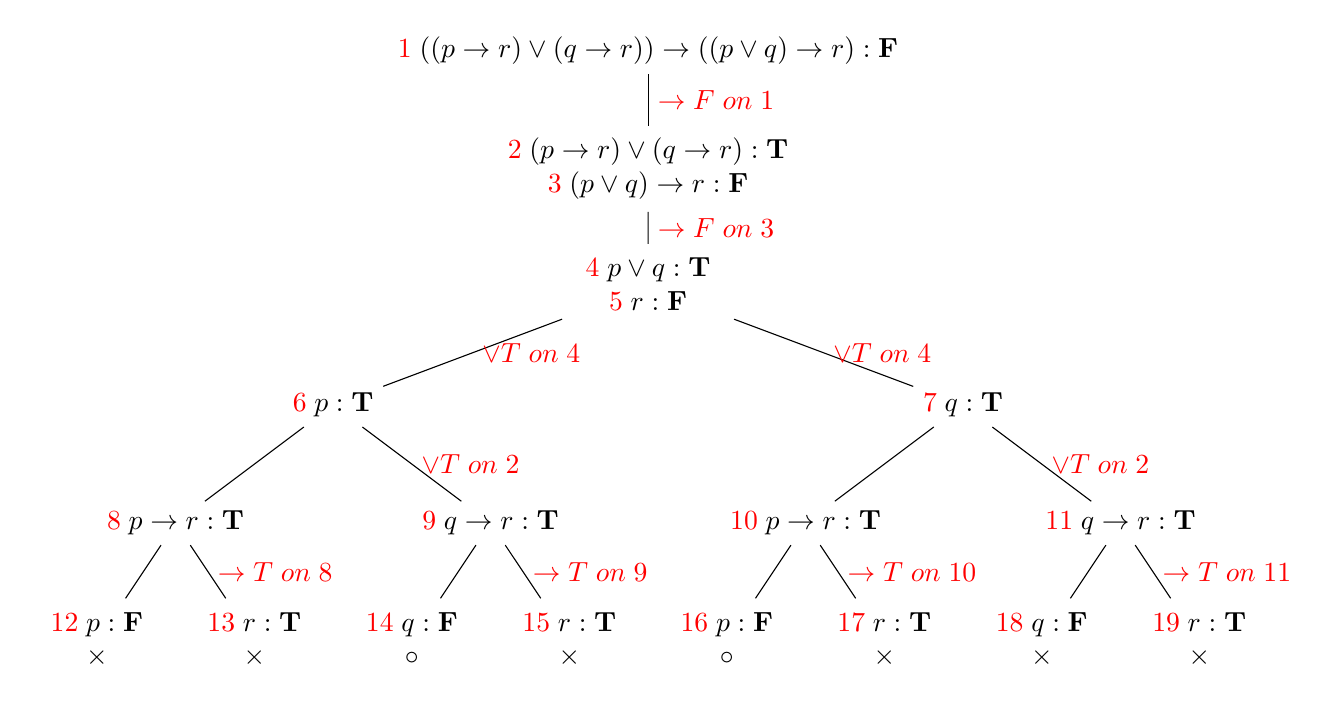
\begin{tikzpicture}

\node {$ \textcolor{red}{1}\; ((p \to r)\lor(q \to r))\to((p \lor q)\to r):\textbf{F} $} [sibling distance = 2.5cm]
        child {node {$ \begin{array}{c} \textcolor{red}{2}\; (p \to r)\lor(q \to r):\textbf{T} \\ \textcolor{red}{3}\; (p \lor q)\to r:\textbf{F} \end{array} $}  
            child {node {$ \begin{array}{c} \textcolor{red}{4}\; p \lor q:\textbf{T} \\ \textcolor{red}{5}\; r:\textbf{F} \end{array} $} [sibling distance = 8cm]
                child {node {$ \textcolor{red}{6}\; p:\textbf{T} $} [sibling distance = 4cm]
                    child {node {$ \textcolor{red}{8}\; p \to r:\textbf{T} $} [sibling distance = 2cm]
                        child {node {$ \begin{array}{c} \textcolor{red}{12}\; p:\textbf{F} \\ \times \end{array} $}}
                        child {node {$ \begin{array}{c} \textcolor{red}{13}\; r:\textbf{T} \\ \times \end{array} $}
                        edge from parent node [right, red] {$\to T\;on\; 8$}}} 
                    child {node {$ \textcolor{red}{9}\; q \to r:\textbf{T} $} [sibling distance = 2cm]
                        child {node {$ \begin{array}{c} \textcolor{red}{14}\; q:\textbf{F} \\ \circ \end{array} $}}
                        child {node {$ \begin{array}{c} \textcolor{red}{15}\; r:\textbf{T} \\ \times \end{array} $ }
                        edge from parent node [right, red] {$\to T\;on\; 9$}}
                        edge from parent node [right, red] {$\lor T\;on\; 2$}}
                        edge from parent node [right, red] {$\lor T\;on\; 4$}}
                child {node {$ \textcolor{red}{7}\; q:\textbf{T} $} [sibling distance = 4cm]
                    child {node {$ \textcolor{red}{10}\; p \to r:\textbf{T} $} [sibling distance = 2cm]
                        child {node {$ \begin{array}{c} \textcolor{red}{16}\; p:\textbf{F} \\ \circ \end{array} $}}
                        child {node {$ \begin{array}{c} \textcolor{red}{17}\; r:\textbf{T} \\ \times \end{array} $}
                        edge from parent node [right, red] {$\to T\;on\; 10$}}} 
                    child {node {$ \textcolor{red}{11}\; q \to r:\textbf{T} $} [sibling distance = 2cm]
                        child {node {$ \begin{array}{c} \textcolor{red}{18}\; q:\textbf{F} \\ \times \end{array} $}}
                        child {node {$ \begin{array}{c} \textcolor{red}{19}\; r:\textbf{T} \\ \times \end{array} $ }
                        edge from parent node [right, red] {$\to T\;on\; 11$}}
                        edge from parent node [right, red] {$\lor T\;on\; 2$}}
                        edge from parent node [right, red] {$\lor T\;on\; 4$}}
                        edge from parent node [right, red] {$\to F\;on\; 3$}} 
                        edge from parent node [right, red] {$\to F\;on\; 1$}};

\end{tikzpicture}
\end{center}

